\documentclass[twocolumn]{article}
\usepackage{authblk}
\usepackage{blindtext}
\usepackage{multicol}% http://ctan.org/pkg/multicols
\usepackage{graphicx}
\usepackage{subcaption}
\usepackage{cite}
\usepackage[table,xcdraw]{xcolor}
\newcommand{\FA}[1]{\begingroup\color{magenta}#1\endgroup}
\newcommand{\TODO}[1]{\begingroup\color{red}#1\endgroup}
%opening
\begin{document}


\title{\textit{MSF: Modulated Sub-graph Finder} }

\author[1]{Mariam R Farman}
\author[1,2]{Fabian Amman}
\author[1]{Ivo L Hofacker}
\affil[1]{Institute for Theoretical Chemistry,Theoretical Biochemistry Group,University of Vienna,Austria}
\affil[2]{Department of Chromosome Biology, Max F. Perutz Laboratories,University of Vienna,Austria}



\maketitle

\begin{abstract}
Differentially expressed genes play an important role in giving
insights to a phenotype. These DEGs are then used to identify the
pathways altered during changing biological conditions. We developed a
novel approach to find the maximal significantly dis-regulated
sub-graphs or cluster of genes from the cell signaling network, giving
these sub-graphs an overall significance of modulation by combining the
individual \textit{p}-values of the genes.
\end{abstract}

\section*{Keywords}

Differentially expressed genes, Pathway analysis, Combining \textit{p}-value, Cell signaling network, Modulated Sub-graphs


\section*{Background}

High throughput sequencing techniques have been widely used to yield
the differentially expressed genes (DEG)~\cite{DEG}. To this end,
changes in transcript abundance are measured, e.g.~by next generation
sequencing techniques, and interpreted as an indicator of differential
expression of genes. DEGs can be used to get
insights into the mechanism underlying differences between conditions of samples, such as
healthy versus diseased. Differential gene
expression analysis (DGEA) informs about the magnitude of expression changes
between the conditions which are the log fold change, the sign of log fold change and the confidence level
of observing a authentic change, often expressed as
\textit{p}-value. These DEGs are
then used to extract meaningful insights, for example the genes that
could be important for a particular condition or maybe the target gene
of any infection or disease. Out of all high throughput analysis
methods currently in use, pathway-based analysis has become an
important tool to further interpret the results of a DGEA and to
acquire understandings of the perturbations in a biological
system. Biological pathways are sets of genes contained in a functional
unit. DEGs help to identify pathways or networks that may be altered
during a change of condition providing important information about
diseases and its treatment process~\cite{Khatri2012}. Pathway-based
methods use the predefined pathways or networks such as
KEGG~\cite{Kegg} and Reactome~\cite{Reactome}, the expression
measurements of the genes obtained from DGEA in combination with statistical methods and algorithms to
identify specifically modulated pathways and processes~\cite{Campos}.

KEGG (Kyoto Encyclopedia of Genes and Genomes) is a database resource for understanding the functionality and utilities of the biological system. KEGG pathways is a branch of KEGG database that has a collection of manually drawn pathway maps representing the molecular interaction, reaction and relation networks of cellular functions. Similarly Reactome is an open-source manually curated, peer-reviewed and well known  database for biological processes pathway.

Existing pathway-based analysis approaches use different research
designs, which can be categorized into ORA (Over-representation
analysis), FCS (Functional class scoring) and pathway topology based
methods. ORA is the first and the most basic method of pathway
analysis. It uses a user defined cut-off for the log-fold change and
\textit{p}-value from the DGEA (most commonly using absolute log-fold change
$\geq$ 2 and \textit{p}-value $\leq$ 0.05) to define a list of
DEGs. Subsequently, sets of genes associated
with annotated pathways are tested for being overrepresented in the
set of DEGs. To this end, hypergeometric
distribution, chi-square tests, binomial probability or the Fisher’s
exact test are used. Thereby the information of the topology of genes in the
pathways are ignored~\cite{Bayer}. Futhermore, ORA assumes that the biological
pathways are independent of each other and ignores the fact that they cross-talk and overlap~\cite{Khatri2012,Campos}.

Unlike ORA, FCS has no artificial cut-off to define DEG list and does
not assume genes to be independent of each other. FCS works in three
step, first it calculates the gene-level statistics including correlation of molecular measurements  using differential expression of individual genes. In the second step the statistics of individual genes are transformed to an individual pathway-level statistic and finally the
pathway-level statistics are accessed. Although FCS covers some of the
limitations from ORA, it still lacks the topology, cross-talk and
overlap of the pathways~\cite{Khatri2012,Campos}. Pathway topology
based methods are similar to FCS except that they consider the
topology of each gene during the gene-level
statistics but still are unable to link different pathways~\cite{Khatri2012}.

On these grounds we propose a novel approach to make use of the rich
pathway annotation resources available to gain additional functional
insights from basic DGEA. To this, we
start with the presupposition that expression of neighboring genes
within a functional pathway are not independent from each
other. Rather, they are often regulating each others expression or are
part of the same regulon~\cite{Michalak}. We
understand that the categorization of links between genes into labeled
pathways is often an arbitrary one, given the extensive cross talk
between different pathways. Although these categories have proven to be
useful in many situations, they force a certain perspective onto the
interpretation of novel data. Based on this two principles, we aim to
find sub-graphs within predefined networks which exhibit as a whole
significant differential expression changes. As input, information on
functional links between genes provided by e.g. KEGG or Reactome and
information on the differential expression status of single genes
resulting from a DGEA, are required. As a result the analysis returns
sub-graphs and their joint confidence scores, reflecting how the
perturbation is migrated through the network. Furthermore, the entry
points of perturbation in the networks and overlap with conventional
pathway categories are returned. All of this can be helpful to
understand the cause end effect of a stimulus and might inform about
potential points of intervention. The proposed algorithm was
implemented as a java program, which was named Modulated Sub-graph
Finder (\texttt{MSF}).

\section*{Methods}
\texttt{MSF} is developed as a novel heuristic approach in Java to
find the modulated sub-graphs of gene interactions from the cell
signaling network. \texttt{MSF} does not work on predefined pathways but builds up the sub-graph from scratch using the whole cell signaling network. The network has nodes corresponding to genes and
edges representing their interactions. 

\texttt{MSF} uses the individual gene's \textit{p}-values generated
from the DGEA. The \textit{p}-value
expresses the probability that the hypothesis of unmodified gene
expression can be rejected for a given statistical model. To find
significantly modulated sub-graphs individual \textit{p}-values of the
vicinal genes in the global network are combined into a single
combined \textit{p}-value, using a statistical method for combining
dependent \textit{p}-values described by Hartung~\cite{Hartung}. Using the inverse of standard normal distribution function $\Phi^{-1}$, individual gene \textit{p}-values $p_i$ are
first transformed to their corresponding normal score $t_i(i=1,...,N)$
\[ t_i = \Phi^{-1}(p_i) \]  

Then using these normal scores, the correlation \textit{Cov} between genes is calculated, 

\[ Cov (t_i, t_j) =\varrho\]

The normal scores, correlations and the correction of correlation are applied to
the inverse normal function to calculate the individual
\textit{p}-value for a sub-graph \textit{Cp}. \newline

$  {\scriptstyle Cp(\varrho,k) = \frac{\sum_{i=1}^{n} \lambda_i t_i}{\sqrt{\sum_{i=1}^{n} \lambda_i^2 +[(\sum_{i=1}^{n} \lambda_i)^2- \sum_{i=1}^{n} \lambda_i^2]\{\varrho+k\cdot\sqrt{\frac{2}{n+1}} (1-\varrho)\}}}} $\\ \newline

Lambda $\lambda$ are the weights for each gene and \textbf{k} is the correction of the correlation. For the moment, equal weights are given to all genes and \textbf{k} used is 0.2 as used by authors. An
overall \textit{p}-value of a sub-graph will express the significance
of all genes in the sub-graph being modulated together.

To reduce the complexity to score all possible connected sub-graphs
\texttt{MSF} applies a three steps heuristic as described in the
following.\newline
 
\subsection*{Overview of our method}

The pipeline of identification of modulated sub-graphs from a network by \texttt{MSF} is depicted in
Fig (1).
\newline

\textbf{Initial Modulated sub-graphs}

\texttt{MSF} constructs the first sub-graph starting with the genes
associated with the lowest (most significant) \textit{p}-value from
the network. It tries to extend the
sub-graph to the most significant neighboring gene. A single combined
\textit{p}-value is calculated for the two genes. If the combined
\textit{p}-value is smaller than the minimal individual gene's
\textit{p}-value, the extended sub-graph is accepted. Then the next most significant neighboring gene is added to the sub-graph and the combined \textit{p}-value is calculated, if the new combined \textit{p}-value of three genes is smaller than the combined \textit{p}-value of the first two genes,the extended sub-graph is accepted. This step is iteratively repeated until no further extension is accepted. In this case the process starts over with all remaining genes not yet in a
significantly modulated sub-graph. This step identifies all the trivial
sub-graphs that are modulated in the whole network~(Fig.~1b).\newline

\textbf{Extending Modulated sub-graphs}

In the next step initial modulated sub-graphs are used to check if
they could further be extended beyond the immediate neighborhood.
This is done by testing all possible extension by two genes for
all genes in the sub-graph. Again, this step is iteratively repeated until no
further genes are added to the significant differentially expressed
sub-graphs. This steps bridges small gaps of genes without a clear
differential signal in the DGEA~(Fig.~1c).\newline

\textbf{Merging Modulated sub-graphs}

After detection and extension of the modulated sub-graphs, they are
tested if combined sub-graph score is better than on their own. The merging of the two sub-graphs is done by depth first search, If the two sub-graphs merge with the connector of at most two genes and the
combined \textit{p}-value of the merged sub-graph including the
bridging genes in between is less than the individual
\textit{p}-values of the two sub-graphs, the two sub-graphs are merged
together to one big modulated sub-graph~(Fig.~1d). This step is repeated iteratively until no sub-graphs could be merged.\newline
 
\textbf{Finding Sources \& Sinks}

In a last post processing step \texttt{MSF} identifies the trigger
points of the modulated sub-graphs. These trigger genes are the sources
of the sub-graphs with only outgoing edges. These genes can be
interpreted as the possible entry points of perturbation from where the
stimulus causes downstream effects. In the same spirit the most
downstream genes of the modulated sub-graph are identified and defined
as sinks. Sinks can be interpreted as the effectors where the
integrated information within the signal transduction network is set
to action.


\section*{Results}

\subsection*{Case Study}

To demonstrate the usefulness \texttt{MSF} is applied to RNAseq data
set of primary human monocyte-derived macrophages (MDMs) infected with
Ebola virus~\cite{Olejnik} (GSE84188). Ebola Virus (EBOV)
belongs to the Filoviridea family; filamentous, enveloped and single
stranded RNA viruses. EBOV causes hemorrhagic fever in humans,
inducing the host innate and adaptive immune response to be unable to
control virus infection~\cite{Prins}. Until now there are no approved
antiviral drugs for the treatment of Ebola virus infection~\cite{Konde,Rhein}. 
The initial targets of EBOV are the macrophages and
dendritic immune cells~\cite{Falasca,Rhein}. Ebola Virus inhibits the critical
innate immune response of the host, which includes the activation of
alpha/beta interferon (IFN-$\alpha /
\beta$)~\cite{Prins,Konde,Cardenas}. The Ebola viral protein VP35
targets the host type~I interferon IFN-$\alpha / \beta$ to block the
early antiviral immune response
~\cite{Prins,Konde,Falasca,Cardenas,Olejnik}. It has been proposed
that IFN-$\alpha / \beta$ could be used through clinical trials to
design antiviral drug against Ebola. The aim of testing the EBOV infection data with \texttt{MSF} was to  identify the modulated sub-graphs and check if \texttt{MSF} is able to identify the IFN-$\alpha / \beta$ gene as one of the sources.

The EBOV infection data has three time-points 6 , 24  and 48 hour post infection (hpi). At 6hpi, five modulated sub-graphs were identified. Most of the genes part of the sub-graphs were chemokines (CXCL10, CCL8) and Interleukin genes (IL6, IL27, IL23) which serve as a subset of CD4+ T helper
cells. IFNB1  and IFNA1 were both identified as two of the sources. Most of the sources identified by \texttt{MSF} were type~I interferon induced genes. At 24hpi nine modulated sub-graphs were identified, IFNA1 was identified as one of the sources. For the last time-point again IFNB1 and IFNA1 were identified as the two sources out of the possible sources from seven sub-graphs identified.

As stated earlier IFN-$\alpha / \beta$ could be one of the target
genes of Ebola infection. We were able to successfully identify IFNA1
as a source in all three time-points and INFB1 in two of the time-points. Although IFNA1 and IFNB1 were two of the most
significant gene in the later time points, \texttt{MSF} was able to detect them as
a source in the early time-point when the genes were not significant
based on the individual DGEA alone. Identifying these sources will reduce the search space for potential target genes and can help the biologist as the starting point of clinical testing for drugs and vaccines against an infection.

\subsection*{Modulated sub-graphs at 6hpi}

 The connected modulated sub-graphs from 6hpi are shown in~(Fig.~2). The graph shows different colors for predefined KEGG pathways and how they cross talk. The KEGG enrichment and visualization on the modulated sub-graph was done using StringApp~\cite{StringApp} in Cytoscape. The graph unveils how more than one stimulus coincide for the progression of infection. The activation of IRF-dependent genes (light Blue), including those for type I IFNs through Toll-like receptor signaling (yellow), exhibits strong inflammatory response as shown by elevated number of inflammatory cytokines and chemokines genes (green and pink). NF-Kappa B activation (off-white) is also mediated by Toll-like receptor. NF-Kappa B signaling is a key regulator of cytokine and chemokine expression\cite{Olejnik}. Toll-like receptor signaling further leads to  MAPK signaling (neon blue), JAK-STAT (red) signaling and TNF signaling (dark blue). Sensor of cytosolic DNA (dark grey) which activates the IRF and NF-Kappa B transcription factors, also leads to production of type I interferon and other cytokines. 
 
 Extracellular matrix (ECM) receptor interaction genes are identified by \texttt{MSF} at the other end of the graph, which are suggested to be in interaction with Ebola glycoprotein (GP)~\cite{Veljkovic}. ECM receptor interactions are seen to lead to Focal adhesion which regulates the P13k-Akt signaling (purple). P13k-Akt signaling goes to FoxO signaling which eventually connects to cell cycle, which at later time-points is disrupted. TNF signaling, P13k-Akt signaling and FoxO signaling activates apoptosis (black) and autophagy. The light gray node belong to other pathways not shown due to graph visual complexity.

 

\subsection*{Comparison} 

To further understand the functional role of the sub-graphs identified by \texttt{MSF}, we linked the  sub-graphs to the predefined KEGG pathways and Reactome
pathways through gene enrichment analysis. We used Cytoscape~\cite{Cyto} plugins to identify the enriched patwhays, CytoKegg~\cite{Cytokegg} for KEGG and Reactome FI~\cite{Reactome} for Reactome. We compared the pathways enriched in \texttt{MSF} identified sub-graphs to pathway analysis by SPIA~\cite{Tarca} for KEGG and Reactome pathway enrichment analysis for Reactome. 

At 6hpi Cytokegg identified the sub-graph genes to be enriched in Toll-like receptor signaling, TNF signaling, IL-17 signaling and NF-kappa signaling pathways, as also stated by~\cite{Olejnik}. The earliest response EBOV induces on cytokine is via TLR4-mediated signaling~\cite{Olejnik}, Gene enrichment analysis of sub-graph genes at 6hpi showed toll-like receptor signaling being most significantly dis-regulated pathway, this important signaling pathway was not identified by SPIA along with RIG-I-like receptor signaling pathway, TNF signaling pathway and IL-17 signaling (Table 1 in the supplement material). On the later time-points \texttt{MSF} and SPIA showed consensus on the important pathways e.g Chemokine signaling, Cytokine-Cytokine receptor interaction, NF-kappa B signaling, Cytosolic DNA-sensing and RIG-I-like receptor signaling as being dis-regulated (Table 2-3 in the supplement). 

Likewise we compared gene enrichment results of sub-graph genes identified by \texttt{MSF} using Reactome FI to the Reactome predefined pathway enrichment analysis. Although \texttt{MSF} and Reactome showed good agreement on the dis-regulated pathways e.g Signaling by Interleukins, Interleukin-10 signaling, Cytokine Signaling in Immune system, Chemokine receptors bind chemokines, RIG-I/MDA5 mediated induction of IFN-alpha/beta pathways, NF-kB activation, Reactome as well could not identify Toll-like receptor signaling (Table 1-3 in the supplement material) . This shows that \texttt{MSF} is able to identify the important modulated genes in the sub-graphs at the earliest time-point of infection.

\subsection*{Robustness}

To assess the robustness and stability of our method, Poisson distributed noise was added to the sample read counts. Then DGEA was carried out on the disturbed data with the same parameters as for the native data, followed by analysis with \texttt{MSF}. Using this criteria, the goal was to spot almost
identical modulated sub-graphs in the real and noisy data. This procedure was carried out 100 times and every time the genes from the sub-graphs identified from noisy data were compared to the genes of sub-graphs identified from the native data. This was also done for the DEG obtained for each run, a cutoff was used to compare the retrieved DEG from noisy data to the native data.  The robustness of \texttt{MSF} and the DEG analysis for the three time-points are shown in~(Fig.~3). We were very stringent in adding noise to the counts, which could be seen by the DEG analysis robustness. For the last time-point (48hpi) 84\% genes of the sub-graphs from native data were retrieved, for 24hpi robustness was about 79\%. Robustness was 71\% at 6hpi, this could be due to that the infection merely started and the signal transdcution was weak as compared to the later time-points.

Simulation testing was also conducted on \texttt{MSF}, the objective was to find less sources than observed in the sub-graphs identified by \texttt{MSF} from native data. Simulation results showed a chance of less than 10 percent to get more sources than observed.


\section*{Discussion}

The discussion should include the implications of the article results
in view of prior work in this field.

\section*{Conclusions}

\textbf{MSF} is a fast and robust tool to find modulated sub-graphs from a given network. So far, it is the only tool from existing approaches that builds the modulated sub-graph from scratch using the network and DEG, where the predefined pathways could be seen connected to each other. The Robustness analysis shows that \textbf{MSF} is robust against noise and thus finds core modulated sub-graphs even if the DGEA is not carried out vigilantly. Alongside with \textbf{MSF}, we provide a good directed cell signaling network file, which is a subset of interactions from Reactome Functional interactions (FIs)
Version 2016 .

\subsection*{Source of data}

The Ebola infection RNAseq dataset analyzed during the current study are
available in the GEO repository (GSE84188). The cell signaling
network file used is from Reactome Functional interactions (FIs)
Version 2016


\subsection*{Author contributions}
FA proposed the idea. MF implemented the method. MF designed the benchmark
data set. MF analyzed the benchmark results. MF, FA, and IH contributed to
the manuscript writing. MF produced all figures. All authors read and
approved the final manuscript.

\subsection*{Competing interests}

The authors declare that they have no competing interests.


\subsection*{Grant information}

This work was funded by the FWF (“Fonds zur Forderung der wissenschaftlichen Forschung”) within the project Internationalen Kooperationsprojektes - Intl cooperation Project (Joint Project - Lead Agency Verfahren) with the project number (I 1988-B22). The grant was assigned to Ivo Hofacker


\subsection*{Acknowledgements}

We thank all our colleagues who provided insight and expertise that greatly assisted the research and all reviewers for their constructive criticism.  

\subsection*{Supplementary Material}

The supplementary file contains tables of comparison between \textbf{MSF} identified sub-graph gene enrichment with SPIA and Reactome pathway analysis. 
\clearpage


\begin{thebibliography}{9}
	 
	\bibitem{DEG}
	Malone, J. H., \& Oliver, B. (2011). Microarrays, deep sequencing and the true measure of the transcriptome. BMC Biology, 9(1), 34. doi:10.1186/1741-7007-9-34
	\bibitem{Khatri2012}
	Khatri, P., Sirota, M., \& Butte, A. J. (2012). Ten Years of Pathway Analysis: Current Approaches and Outstanding Challenges. PLoS Computational Biology, 8(2). doi:10.1371/journal.pcbi.1002375
	\bibitem{Kegg}
	Kanehisa, M. (2000). KEGG: Kyoto Encyclopedia of Genes and Genomes. Nucleic Acids Research, 28(1), 27-30. doi:10.1093/nar/28.1.27
	\bibitem{Reactome}
	Croft, D., \& Croft, D. (2010). Reactome: A database of biological pathways. Nature Precedings. doi:10.1038/npre.2010.5025
	\bibitem{Campos}
	García-Campos, M. A., Espinal-Enríquez, J., \& Hernández-Lemus, E. (2015). Pathway Analysis: State of the Art. Frontiers in Physiology, 6. doi:10.3389/fphys.2015.00383 
	\bibitem{Bayer}
	Bayerlová, M., Jung, K., Kramer, F., Klemm, F., Bleckmann, A., \& Beißbarth, T. (2015). Comparative study on gene set and pathway topology-based enrichment methods. BMC Bioinformatics, 16(1). doi:10.1186/s12859-015-0751-5   
	\bibitem{Hartung}
	Hartung, J. (1999). A Note on Combining Dependent Tests of Significance. Biometrical Journal, 41(7), 849-855. doi:10.1002/(sici)1521-4036(199911)41:7<849::aid-bimj849>3.0.co;2-t 5 
	
	\bibitem {Prins}
	Prins, K., Cardenas, W. and Basler, C. (2009). Ebola Virus Protein VP35 Impairs the Function of Interferon Regulatory Factor-Activating Kinases IKK and TBK-1. Journal of Virology, 83(7), pp.3069-3077.
	
	\bibitem {Konde}
	Konde, M., Baker, D., Traore, F., Sow, M., Camara, A., Barry, A., Mara, D., Barry, A., Cone, M., Kaba, I., Richard, A., Beavogui, A., Günther, S., Pintilie, M. and Fish, E. (2017). Interferon β-1a for the treatment of Ebola virus disease: A historically controlled, single-arm proof-of-concept trial. PLOS ONE, 12(2).
	
	\bibitem {Rhein}
	Rhein, B., Powers, L., Rogers, K., Anantpadma, M., Singh, B., Sakurai, Y., Bair, T., Miller-Hunt, C., Sinn, P., Davey, R., Monick, M. and Maury, W. (2015). Interferon-γ Inhibits Ebola Virus Infection. PLOS Pathogens, 11(11), p.e1005263.
	
	\bibitem {Falasca}
	Falasca, L., Agrati, C., Petrosillo, N., Di Caro, A., Capobianchi, M., Ippolito, G. and Piacentini, M. (2015).
	 Molecular mechanisms of Ebola virus pathogenesis: focus on cell death. Cell Death and Differentiation, 22(8), pp.1250-1259.
	 
	\bibitem {Cardenas}
	Cardenas, W., Loo, Y., Gale, M., Hartman, A., Kimberlin, C., Martinez-Sobrido, L., Saphire, E. and Basler, C. (2006). Ebola Virus VP35 Protein Binds Double-Stranded RNA and Inhibits Alpha/Beta Interferon Production Induced by RIG-I Signaling. Journal of Virology, 80(11), pp.5168-5178.
	
	\bibitem {Olejnik}
	Olejnik, J., Forero, A., Deflubé, L., Hume, A., Manhart, W., Nishida, A., Marzi, A., Katze, M., Ebihara, H., Rasmussen, A. and Mühlberger, E. (2017). Ebolaviruses Associated with Differential Pathogenicity Induce Distinct Host Responses in Human Macrophages. Journal of Virology, 91(11), pp.e00179-17.
	
	\bibitem {Dilley}
	Dilley, K., Voorhies, A., Luthra, P., Puri, V., Stockwell, T., Lorenzi, H., Basler, C. and Shabman, R. (2017). The Ebola virus VP35 protein binds viral immunostimulatory and host RNAs identified through deep sequencing. PLOS ONE, 12(6), p.e0178717.
	

	\bibitem{Michalak}
	Michalak, P. (2008). Coexpression, coregulation, and cofunctionality of neighboring genes in eukaryotic genomes. Genomics, 91(3), 243-248. doi:10.1016/j.ygeno.2007.11.002 
	
	\bibitem{Cyto}
	http://www.cytoscape.org/
	
	\bibitem{Cytokegg}
	http://apps.cytoscape.org/apps/cytokegg
	
	\bibitem{Reactome}
	https://wiki.reactome.org/index.php?title=ReactomeFIViz
	
	\bibitem{Tarca}
	Tarca, A. L., Draghici, S., Khatri, P., Hassan, S. S., Mittal, P., Kim, J., … Romero, R. (2009). A novel signaling pathway impact analysis. Bioinformatics, 25(1), 75–82. http://doi.org/10.1093/bioinformatics/btn577
	
	\bibitem{StringApp}
	http://apps.cytoscape.org/apps/stringapp
	
	\bibitem{Veljkovic}
	Veljkovic, V., Glisic, S., Muller, C. P., Scotch, M., Branch, D. R., Perovic, V. R., … Colombatti, A. (2015). In silico analysis suggests interaction between Ebola virus and the extracellular matrix. Frontiers in Microbiology, 6, 135. http://doi.org/10.3389/fmicb.2015.00135
	
	
\end{thebibliography}



\begin{figure*}[ht!]
		\centering
	\fbox{
		\begin{minipage}{17 cm}
	
	\begin{subfigure}{.5\textwidth}
		\centering
		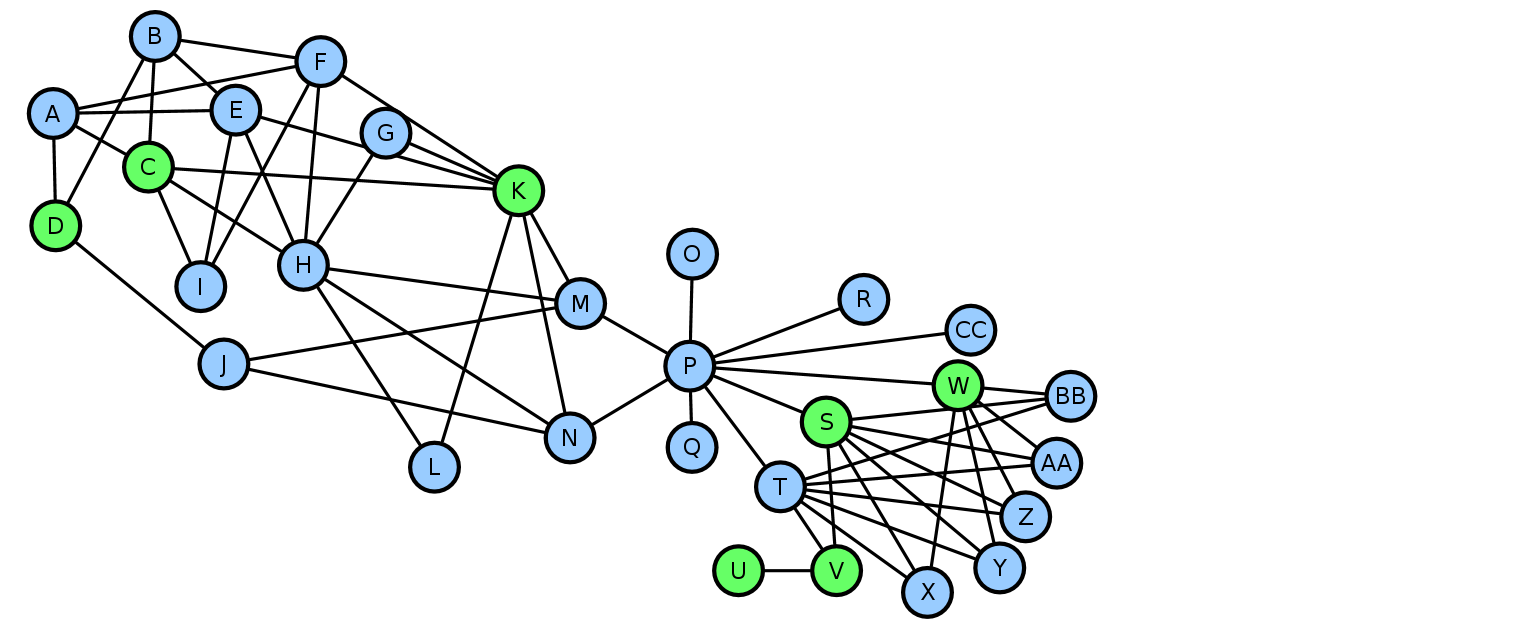
\includegraphics[width=10.0cm]{Documents/PhDThesis/MSFPaper/Tgfb1} 
		\caption{}
	\end{subfigure}
	\begin{subfigure}{.5\textwidth}
		\centering
		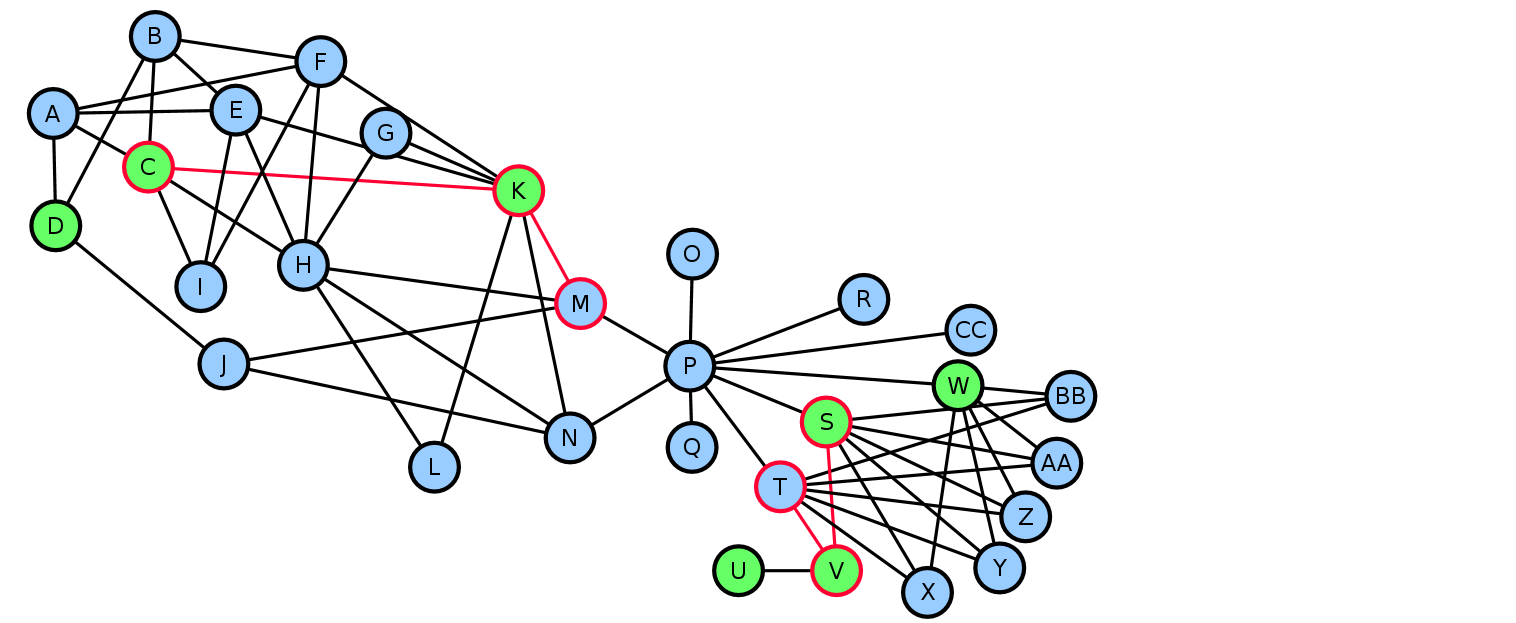
\includegraphics[width=10.0cm]{Documents/PhDThesis/MSFPaper/TGFBstep1}
		\caption{}
	\end{subfigure}
	\begin{subfigure}{.5\textwidth}
		\centering
		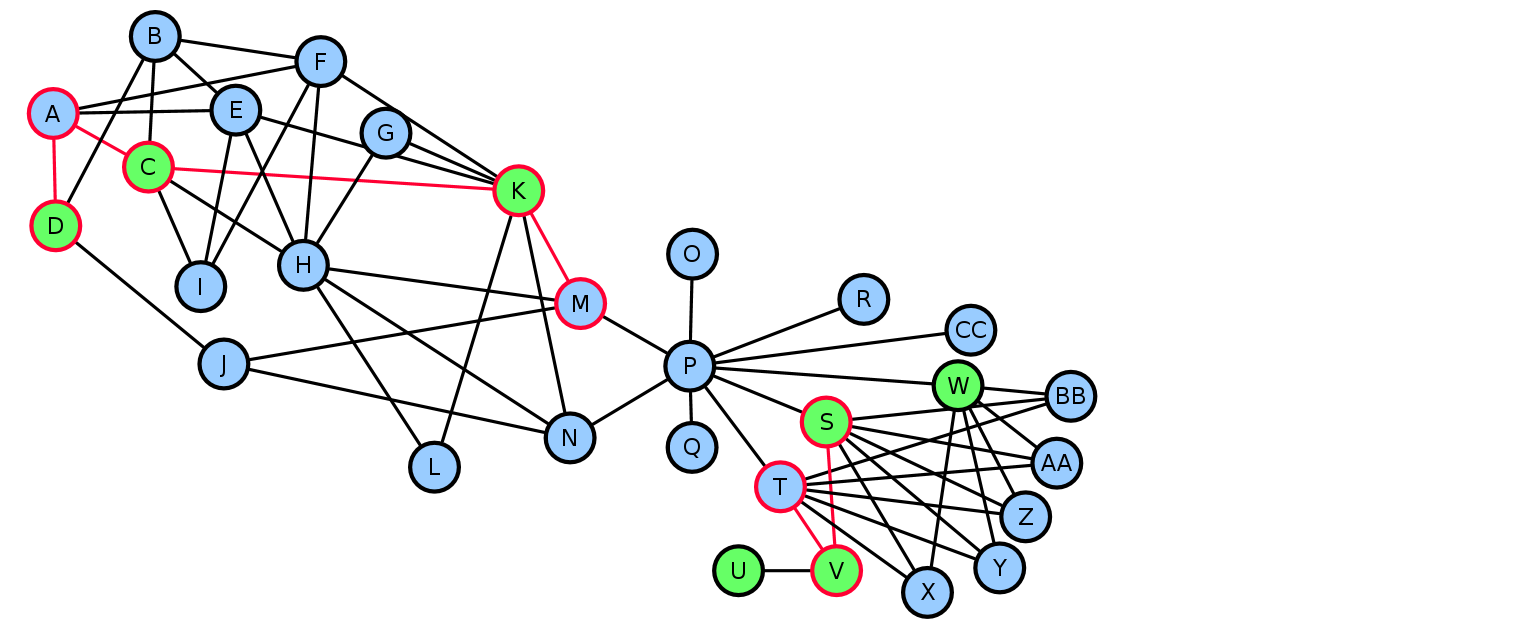
\includegraphics[width=10.0cm]{Documents/PhDThesis/MSFPaper/TGFBstep2} 
		\caption{}
	\end{subfigure}
	\begin{subfigure}{.5\textwidth}
		\centering
		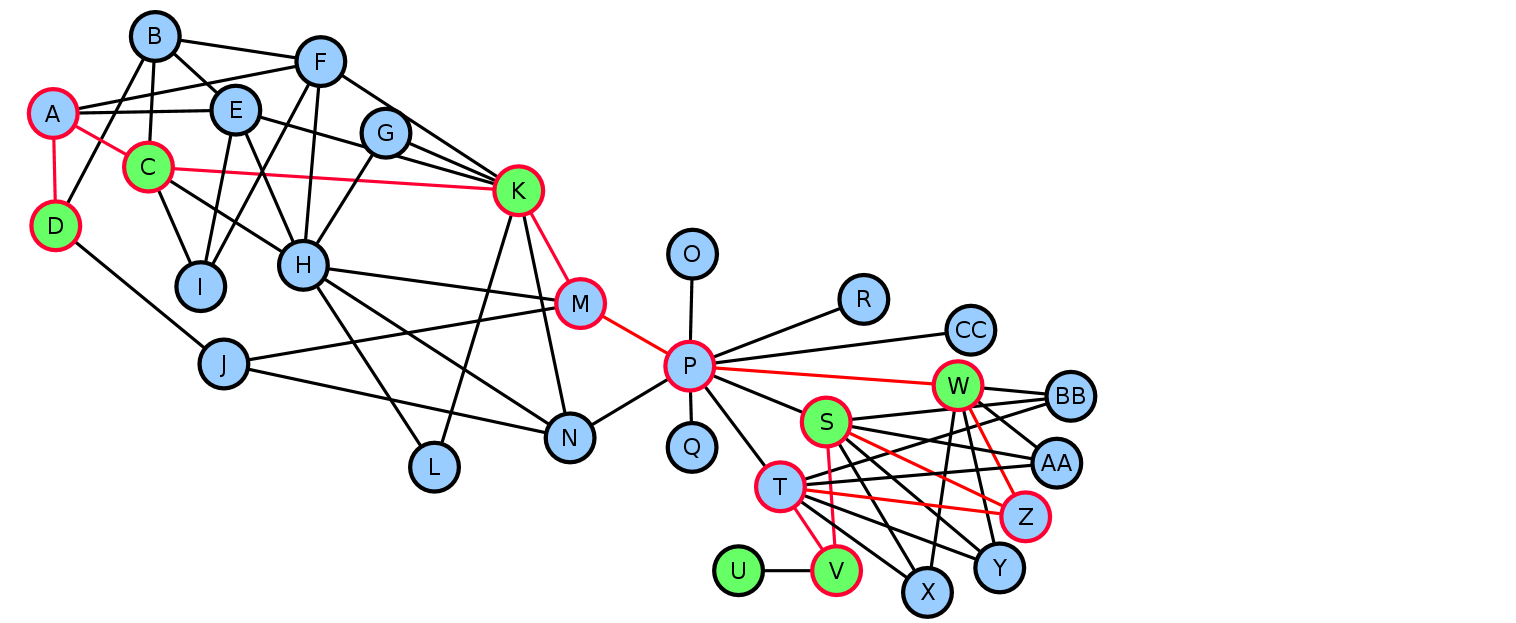
\includegraphics[width=10.0cm]{Documents/PhDThesis/MSFPaper/TGFBstep3}
		\caption{}
	\end{subfigure}
	\caption{Overview of \texttt{MSF} process showing the steps to identify the modulated sub-graphs. (a) showing a network of genes with green nodes as genes with \textit{p}-values $< $ 0.05, and blue nodes are genes with \textit{p}-values $>$ 0.05, (b) the genes circled red show the two initial modulated sub-graphs, sub-graph1 found one with M,K,C and the second modulated sub-graph2 S,V,T, (c) shows the modulated sub-graph1 being extended to M,K,C,A,D, (d) shows both the modulated sub-graphs merged with the addition of 3 genes Z,W,P.}
			\end{minipage}
}
\end{figure*}

\begin{figure*}
	\centering
	\fbox{
		\begin{minipage}{17 cm}
	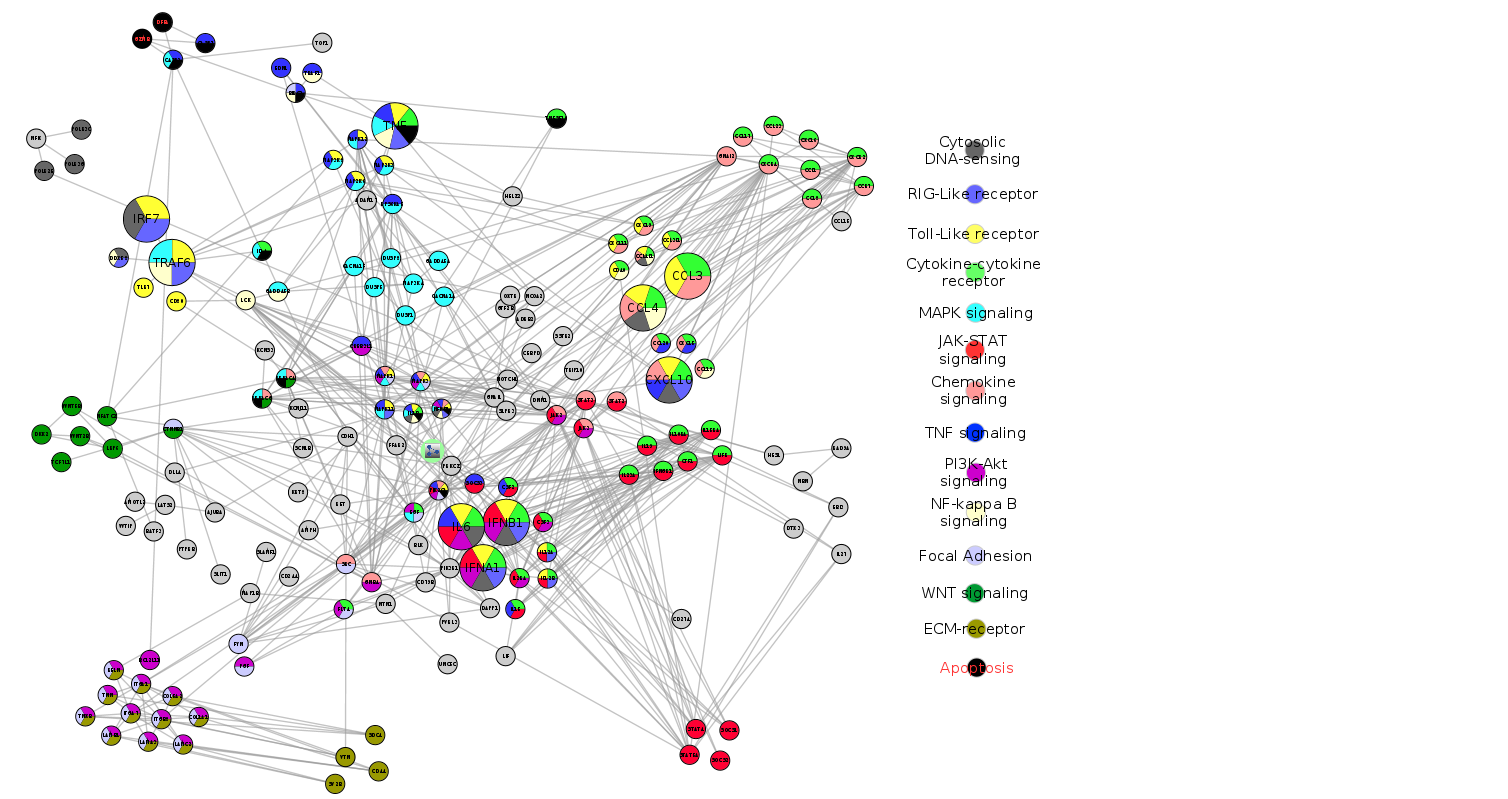
\includegraphics[width=1.4\linewidth]{ModulatesSubPaths/MSFData/Ebola6H/newestMergedNetwork}
	\caption{Shows connected modulated sub-graphs from 6hpi, where nodes are genes and edges are the interactions. The node coloring represents the predefined KEGG pathways referring to the nodes in the legend, the edges are from Reactome. Important genes to EBOV infection as from literature are enlarged in the graph. The signal flow depicted in the graph is explained in the text.}
		\end{minipage}
}
\end{figure*}

\begin{figure*}[p]
	\centering
	\fbox{
		\begin{minipage}{17 cm}
			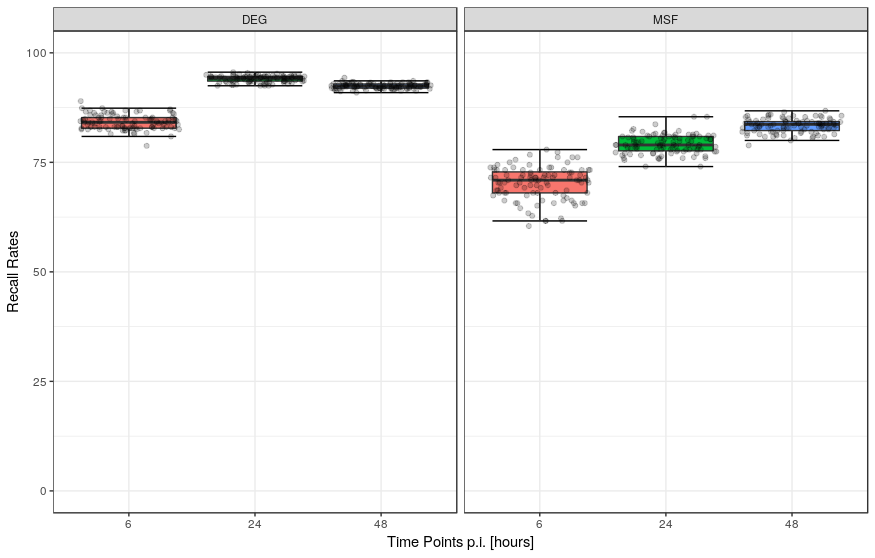
\includegraphics[width=16cm]{Documents/PhDThesis/MSFPaper/DEGvsMSF2}
			\caption{Graph shows the percentage of DEG analysis genes and MSF identified sub-graph genes recall rates 100 times for the three different time points after the addition of Poisson distributed noise.}
			\label{label}
		\end{minipage}
	}
\end{figure*}




\end{document}
